\documentclass[12pt,svgnames]{extarticle}

% Physical poster canvas: portrait A1 without an implicit content margin.
\usepackage[a1paper,margin=0mm]{geometry}

\DeclareTextCommandDefault{\nobreakspace}{\leavevmode\nobreak\ }

% --- Enable notes ---
% \setbeameroption{show notes} % allow \note{} content

% --- Show notes on second screen (right of main slides) ---
% \setbeameroption{show notes on second screen=right}

\usepackage{xcolor}
\usepackage{listings}
\usepackage[english]{babel}
\usepackage{fontspec}

\usepackage{amsmath}
\usepackage{amssymb}
\usepackage{siunitx}
\usepackage{pifont}
\usepackage{caption}


\usepackage{tikz}
\usepackage{tikzpagenodes}
\usetikzlibrary{shapes,calc,decorations.pathreplacing,decorations.pathmorphing,arrows.meta,shapes.geometric,shapes.callouts}
\usetikzlibrary{positioning,fit,patterns,trees,backgrounds,matrix,overlay-beamer-styles,tikzmark,fadings}
 
% Shared palette, derived from the grid-index figures.
\definecolor{color1}{HTML}{4357AD}
\definecolor{color2}{HTML}{48A9A6}
\definecolor{color3}{HTML}{E4DFDA}
\definecolor{color4}{HTML}{D4B483}
\definecolor{color5}{HTML}{C1666B}

\def\pagecolor{color4}
\def\cellcolor{black}
\def\pagebuffercolor{color4}
\def\volumecolor{color2}
\def\imbalancecolor{color4}
\def\overheadcolor{color5}
\def\ttopacity{1}

\tikzset{
  my callout style/.style={
    draw=none, rectangle callout, anchor=pointer,
    callout relative pointer={(320:1.5cm)},
    rounded corners, align=center, opacity=\ttopacity
  },
  overlay callout/.style={
    draw=none, rectangle callout,
    callout relative pointer={(320:1.5cm)},
    rounded corners, align=center, opacity=\ttopacity
  },
  iconW/.store in=\iconW, iconW=4cm,
  iconH/.store in=\iconH, iconH=4cm,
  barrel/.style={
    draw, gray!70!black, fill=\volumecolor,
    shape=cylinder, shape border rotate=90,
    aspect=0.35, minimum width=9mm, minimum height=11mm, line width=0.6pt
  },
  leafbox/.style={
    draw=gray!70!black, fill=\overheadcolor, rounded corners=0.9pt,
    minimum width=4mm, minimum height=4mm, line width=0.5pt
  },
  gridcell/.style={
    draw=gray!70!black, fill=color3, rounded corners=0.9pt,
    minimum width=4mm, minimum height=4mm, line width=0.5pt
  },
  beam/.style={line width=0.9pt},
  loadL/.style={
    draw=gray!70!black, fill=\imbalancecolor, line width=0.6pt,
    minimum width=8mm, minimum height=7mm
  },
  loadR/.style={
    draw=gray!70!black, fill=\imbalancecolor, line width=0.6pt,
    minimum width=5mm, minimum height=5mm
  },
  fulcrum/.style={draw, fill=black!15, line width=0.6pt},
  iconbox/.style={
    minimum width=\iconW, minimum height=\iconH,
    inner sep=0, outer sep=0, draw=none
  },
  halo arrow/.style={
    ->, >=Stealth, line width=2pt, draw=black, line cap=round
  }
}

\usepackage{mathspec}
\usepackage{lmodern}

%% use Source Sans font
\setmainfont{Source Sans Pro}

%%----------------------%%
%% TikZ                 %%
%%----------------------%%
\usepackage{tikz}
\usetikzlibrary{plotmarks}
\usetikzlibrary{shadows}
\usetikzlibrary{positioning}
\usetikzlibrary{patterns}
\usetikzlibrary{topaths}
%\usetikzlibrary{automata}
\usetikzlibrary{decorations.pathreplacing}
\usetikzlibrary{decorations.text}
\usetikzlibrary{fadings}
\usetikzlibrary{calc}
\usetikzlibrary{snakes}
\usetikzlibrary{shapes.callouts}
\usetikzlibrary{shapes.arrows}
\usetikzlibrary{shapes.geometric}
\usetikzlibrary{arrows}
\usetikzlibrary{arrows.meta}


\usepackage{paralist}
\usepackage{amssymb}

\usepackage{colortbl}

\usepackage{nicefrac}

\usepackage{fancyvrb}

%%----------------------%%
%% PGF Plots            %%
%%----------------------%%
\usepackage{pgfplotstable}
\usepackage{pgfplots}

% no page numbers
\pagestyle{empty}

%%----------------------%%
%% Colors               %%
%%----------------------%%
\definecolor{TuDoGreen}{cmyk}{.57,0,1,0}


\newcommand{\greencirc}[1]{%
  \tikz[baseline=0pt]
    \node[white, circle, fill=TuDoGreen, inner sep=1pt, text height=1.5ex,
          anchor=base]
      { \makebox[0pt]{\smash{\raisebox{.15ex}{#1}}} };%
}

\colorlet{structure}{TuDoGreen}

\tikzset{snake it/.style={decorate, decoration=snake}}

% \newcommand{\itemdot}{\textcolor{TuDoGreen}{$\bullet$}}
% \newcommand{\itemtriangle}{\textcolor{TuDoGreen}{$\RHD$}}
% \newcommand{\itemarrow}{\textcolor{TuDoGreen}{$\rightarrow$}}

\newcommand{\PanelHeadingFont}{\fontsize{30pt}{36pt}\selectfont}
\newcommand{\PosterTitleFont}{\fontsize{54pt}{60pt}\selectfont}
\newcommand{\PosterAuthorFont}{\fontsize{28pt}{34pt}\selectfont}
\newcommand{\PanelHeading}[1]{{\PanelHeadingFont\bfseries #1}}
\newcommand{\HeaderTextColor}{black}

\usepackage{qrcode}

%----------------------%%
% Poster geometry       %%
%----------------------%%
% Adjust these lengths to change the complete layout.  Horizontal placement
% is derived exclusively from \PosterEdgeInset and the individual panel widths.
\newlength{\PosterEdgeInset}
\setlength{\PosterEdgeInset}{20mm}
\newlength{\HeaderHeight}
\setlength{\HeaderHeight}{86mm}
\newlength{\FooterHeight}
\setlength{\FooterHeight}{40mm}
\newlength{\ContentRowHeight}
\setlength{\ContentRowHeight}{165mm}
\newlength{\RowGap}
\setlength{\RowGap}{8mm}
\newlength{\PanelPadding}
\setlength{\PanelPadding}{10mm}
\newlength{\PanelCornerRadius}
\setlength{\PanelCornerRadius}{10mm}
\newlength{\HeaderTopPadding}
\setlength{\HeaderTopPadding}{10mm}
\newlength{\HeaderLogoAreaWidth}
\setlength{\HeaderLogoAreaWidth}{170mm} %% manually set, should account for the full logo to the left
\newlength{\TitleAuthorGap}
\setlength{\TitleAuthorGap}{4mm}
\newlength{\HeaderTextWidth}
\setlength{\HeaderTextWidth}{\dimexpr\paperwidth-\HeaderLogoAreaWidth-\PosterEdgeInset\relax}
\newlength{\ContentWidth}
\setlength{\ContentWidth}{\dimexpr\paperwidth-2\PosterEdgeInset\relax}

% Independently adjustable widths for the two-panel rows.
\newlength{\SettingPanelWidth}
\setlength{\SettingPanelWidth}{190mm}
\newcommand{\SettingPanelContentFont}{\fontsize{20pt}{26pt}\selectfont}
\newlength{\DesignSpacePanelWidth}
\setlength{\DesignSpacePanelWidth}{340mm}
\newlength{\SelectivityPanelWidth}
\setlength{\SelectivityPanelWidth}{240mm}
\newlength{\GridPlanPanelWidth}
\setlength{\GridPlanPanelWidth}{300mm}
\newlength{\DesignSpaceFigureUnit}
\setlength{\DesignSpaceFigureUnit}{19mm}
\newlength{\DesignSpaceFigureTopOffset}
\setlength{\DesignSpaceFigureTopOffset}{25mm}
\newlength{\DesignSpaceFigureContentVerticalShift}
\setlength{\DesignSpaceFigureContentVerticalShift}{15mm}
\newlength{\DesignSpaceFootnoteRightInset}
\setlength{\DesignSpaceFootnoteRightInset}{10mm}
\newlength{\DesignSpaceFootnoteTopInset}
\setlength{\DesignSpaceFootnoteTopInset}{15mm}
\newcommand{\DesignSpaceFigureLabelFont}{\fontsize{16pt}{20pt}\selectfont}
\newcommand{\DesignSpaceFigureTextFont}{\fontsize{18pt}{22pt}\selectfont}
\newcommand{\DesignSpaceFigureEmphasisFont}{\fontsize{24pt}{28pt}\selectfont}
\newlength{\SelectivityFigureUnit}
\setlength{\SelectivityFigureUnit}{17mm}
\newlength{\SelectivityFigureTopOffset}
\setlength{\SelectivityFigureTopOffset}{30mm}
\newcommand{\SelectivityFigureFont}{\fontsize{16pt}{19pt}\selectfont}
\newcommand{\SelectivityResultFont}{\fontsize{13pt}{15pt}\selectfont}
\newlength{\TradeoffFigureWidth}
\setlength{\TradeoffFigureWidth}{165mm}
\newlength{\TradeoffFigureGap}
\setlength{\TradeoffFigureGap}{19.5mm}
\newlength{\TradeoffFigureTopOffset}
\setlength{\TradeoffFigureTopOffset}{45mm}
\newlength{\PerformancePlotWidth}
\setlength{\PerformancePlotWidth}{145mm}
\newlength{\PerformanceFigureTopOffset}
\setlength{\PerformanceFigureTopOffset}{20mm}
\newlength{\PerformancePieWidth}
\setlength{\PerformancePieWidth}{150mm}
\newcommand{\PerformancePuzzleRotation}{-135}
\newcommand{\PerformancePuzzleFont}{\fontsize{5pt}{6pt}\selectfont}
\newcommand{\PerformancePuzzleCenterFont}{\fontsize{6pt}{8pt}\selectfont}
\newcommand{\PerformancePuzzleOuterLabelFont}{\fontsize{7pt}{8pt}\selectfont}
\newlength{\GridFigureTopOffset}
\setlength{\GridFigureTopOffset}{45mm}
\newlength{\GridDataSpaceWidth}
\setlength{\GridDataSpaceWidth}{72mm}
\newlength{\GridFigureWidth}
\setlength{\GridFigureWidth}{160mm}
\newlength{\GridGroupStackXOffset}
\setlength{\GridGroupStackXOffset}{3mm}
\newlength{\GridGroupStackYOffset}
\setlength{\GridGroupStackYOffset}{3mm}
\newlength{\GridCubeLift}
\setlength{\GridCubeLift}{29mm}
\newlength{\GridDataSpaceArrowXOffset}
\setlength{\GridDataSpaceArrowXOffset}{-0.7cm}
\newlength{\GridDataSpaceArrowYOffset}
\setlength{\GridDataSpaceArrowYOffset}{-1.7cm}
\newlength{\PlanXShift}
\setlength{\PlanXShift}{19cm}
\newlength{\PlanFigureUnit}
\setlength{\PlanFigureUnit}{10mm}
% Vertical whitespace between the closest children of adjacent union subtrees.
\newlength{\ComplexPlanBranchGap}
\setlength{\ComplexPlanBranchGap}{5mm}
% Vertical centre-to-centre distance between children of one union subtree.
\newlength{\ComplexPlanLeafGap}
\setlength{\ComplexPlanLeafGap}{3mm}
\newcommand{\ComplexPlanTopChildY}{0.0}
\newcommand{\ComplexPlanUnionSymbol}{$\bigcup$}
\newlength{\SsdReferenceLeafXOffset}
\setlength{\SsdReferenceLeafXOffset}{100.6mm}
\newlength{\SsdReferenceLeafYOffset}
\setlength{\SsdReferenceLeafYOffset}{-107mm}
\newlength{\ComplexPlanSingleLeafXOffset}
\setlength{\ComplexPlanSingleLeafXOffset}{0mm}
\newlength{\ComplexPlanSingleLeafYOffset}
\setlength{\ComplexPlanSingleLeafYOffset}{-10.2cm}
\newlength{\GridPlanGroupBoxPadding}
\setlength{\GridPlanGroupBoxPadding}{3mm}
\newlength{\GridPlanNotesWidth}
\setlength{\GridPlanNotesWidth}{55mm}
\newlength{\GridPlanNotesTopOffset}
\setlength{\GridPlanNotesTopOffset}{5mm}
\newlength{\GridPlanNotesMinHeight}
\setlength{\GridPlanNotesMinHeight}{40mm}
\newcommand{\GridPlanFigureFont}{\fontsize{12pt}{14pt}\selectfont}

\newcommand{\OutlookPuzzleSide}[1]{%
    (-0.55,#1*0.00) .. controls (-0.55,#1*0.00) and (-0.12,#1*-0.05) ..
    (-0.12,#1*0.05) .. controls (-0.12,#1*0.14) and (-0.32,#1*0.30) ..
    (0.0,#1*0.30) .. controls (0.32,#1*0.30) and (0.12,#1*0.14) ..
    (0.12,#1*0.05) .. controls (0.12,#1*-0.05) and (0.55,#1*0.00) ..
    (0.55,#1*0.00)%
}
\newcommand{\OutlookPuzzlePiece}[6]{%
    \path[draw=#1!82!black, fill=#1, line width=1pt, line join=round]
        {[rotate=#2] [shift={(1.10,0)}] \OutlookPuzzleSide{#4}}
        arc[start angle=#2, end angle=#3, radius=1.65]
        {[rotate=#3] [shift={(1.10,0)}] [rotate=180] -- \OutlookPuzzleSide{#5}}
        arc[start angle=#3, end angle=#2, radius=0.55] -- cycle;
    \node[font=\PerformancePuzzleFont\bfseries, text=white, align=center]
        at ({(#2+#3)/2}:1.05) {#6};%
}

% A1 dimensions: twice the source poster's branding dimensions.
\newlength{\TuLogoHeight}
\setlength{\TuLogoHeight}{24mm}
\newlength{\BmftrLogoHeight}
\setlength{\BmftrLogoHeight}{48mm}
\newlength{\LamarrLogoHeight}
\setlength{\LamarrLogoHeight}{28mm}
\newlength{\QrCodeHeight}
\setlength{\QrCodeHeight}{34mm}

\colorlet{HeaderBandColor}{color3!80!white}
\colorlet{FooterBandColor}{color3!80!white}
\colorlet{PanelFillColor}{white}
\colorlet{PanelBorderColor}{color3!10!black}
\colorlet{PerformanceGeneralLabelColor}{color1!90}
\colorlet{PerformanceDomainLabelColor}{color2!90}
\colorlet{PerformanceGeneralPieceColor}{color1!90}
\colorlet{PerformanceDomainPieceColor}{color2!90}

\begin{document}

\begin{tikzpicture}[remember picture, overlay]

    %------- Styles ------%
    \tikzstyle{band} = [anchor=north west, inner sep=0pt];
    \tikzstyle{panel} = [anchor=north west,
        fill=PanelFillColor, draw=PanelBorderColor, line width=1.5pt,
        rounded corners=\PanelCornerRadius, inner sep=0pt];
    \tikzstyle{panel heading} = [anchor=north west, align=left, inner sep=0pt,
        text=black];

    % %------- Background ------%
    % \draw (current page.center) node[opacity=0.5] {%
    %     \includegraphics[height=\paperheight]{figures/die_shot_raptor_big_scale.jpg}
    % };
    
    %------- Header ------%
    \node[band, fill=HeaderBandColor, minimum width=\paperwidth,
        minimum height=\HeaderHeight] (header-band) at (current page.north west) {};
    \node[anchor=west] at ([xshift=\PosterEdgeInset]header-band.west) {
        
\includegraphics[height=\TuLogoHeight]{figures/logo/tud_logo_cmyk}
    };
    % % Calibration guide: this is the remaining header area in which the
    % % title and author block are horizontally centred.
    % \draw[draw=red!80!black, dashed, line width=1pt]
    %     ([xshift=\HeaderLogoAreaWidth]header-band.north west) rectangle
    %     ([xshift=-\PosterEdgeInset]header-band.south east);
    \node[anchor=north west, inner sep=0pt, text width=\HeaderTextWidth,
        font=\PosterTitleFont, text=\HeaderTextColor, align=center] (title)
        at ([xshift=\HeaderLogoAreaWidth,yshift=-\HeaderTopPadding]header-band.north west) { %
        \bfseries Index Intersection for\\%
        \bfseries High-Dimensional Range Queries%
    };
    \node[anchor=north, inner sep=0pt, font=\PosterAuthorFont, text=\HeaderTextColor, align=center]
        at ([yshift=-\TitleAuthorGap]title.south) {%
        Max Berens $\cdot$ Jens Teubner\\%
        DBIS Group, TU Dortmund University%
    };

    %------- Row 1: Setting + Team Composition Design Space ------%
    \node[panel, minimum width=\SettingPanelWidth, minimum height=\ContentRowHeight]
        (setting-panel) at ([xshift=\PosterEdgeInset,yshift=-\RowGap]header-band.south west) {};
    \node[panel heading] (setting-heading)
        at ([xshift=\PanelPadding,yshift=-\PanelPadding]setting-panel.north west) {
        \PanelHeading{Problem Setting}
    };
    \node[anchor=north west, inner sep=0pt]
        at ([yshift=-6mm]setting-heading.south west) {
        \begin{minipage}{\dimexpr\SettingPanelWidth-2\PanelPadding\relax}
            \SettingPanelContentFont
            \begin{itemize}
                \item Scientific data sets, e.g., particle physics or astronomy
                \item High-dimensional, highly selective range queries
                \item Tera/Petabyte scale tables
                \item Scans are infeasible
                \item Traditional indexing fails:
                    \begin{itemize}
                        \item \textbf{1 index per table}: Curse of dimensionality\ldots
                        \item \textbf{1 index per attribute}: High storage costs \& high access volumes\ldots
                    \end{itemize}
            \end{itemize}
            \vspace{1cm}
            {\center \fontsize{24pt}{28pt}\selectfont\textbf{How can we make indexing feasible at scale?}}
            
        \end{minipage}
    };
    \node[panel, anchor=north east, minimum width=\DesignSpacePanelWidth,
        minimum height=\ContentRowHeight] (design-space-panel)
        at ([xshift=-\PosterEdgeInset,yshift=-\RowGap]header-band.south east) {};
    \node[panel heading] at ([xshift=\PanelPadding,yshift=-\PanelPadding]design-space-panel.north west) {
        \PanelHeading{Idea: Generalise Bitmap Indices}
    };
    \node[anchor=north] at ([yshift=-\DesignSpaceFigureTopOffset]design-space-panel.north) {
        \begin{tikzpicture}[x=\DesignSpaceFigureUnit,y=\DesignSpaceFigureUnit]
            \tikzset{
                index label/.style={font=\DesignSpaceFigureLabelFont, align=center},
                index design configuration/.style={rounded corners=4pt, draw=color1, fill=PanelFillColor,
                    line width=0.9pt, inner sep=4pt, font=\DesignSpaceFigureEmphasisFont},
                index design extreme/.style={rounded corners=4pt, draw=color5!90, fill=PanelFillColor,
                    line width=1.3pt, inner sep=4pt, font=\DesignSpaceFigureEmphasisFont, text=black!65},
                index design sublabel/.style={font=\DesignSpaceFigureLabelFont, text=black!55, align=center}
            }
            \def\indexdesignstackspacing{0.55}
            \filldraw[fill=color3!30, draw=color3!60, line width=1.1pt]
                (6.65,3.0) ellipse (7 and 2.25);
            \begin{scope}[yshift=\DesignSpaceFigureContentVerticalShift]
                \node[index design extreme] at (1.45,2.80) {$16 \times 1$};
                \node[index design sublabel] at (1.45,2.12) {1 per table};
                \node[index design extreme] at (11.85,2.80) {$1 \times 16$};
                \node[index design sublabel] at (11.85,2.12) {1 per attribute};
                \node[overlay callout,fill=color2!70,anchor=pointer,
                    callout relative pointer={(265:1.3cm)}, font=\DesignSpaceFigureTextFont] at (11.85,3.10)
                    {``Bitmap index'':\\$\{\{A\}, \{B\}, \ldots, \{P\}\}$};
                \node[overlay callout,fill=color2!70,anchor=pointer,
                    callout relative pointer={(275:1.3cm)}, font=\DesignSpaceFigureTextFont] at (1.45,3.10)
                    {``One big index'':\\$\{\{A, B, \ldots, P\}\}$};
                \node[index design configuration] at (3.85,{2.80 + \indexdesignstackspacing}) {$8 \times 2$\,?};
                \node[font=\DesignSpaceFigureTextFont, text=black] at (3.85,2.85) {$\vdots$};
                \node[index design configuration] at (3.85,{2.80 - \indexdesignstackspacing}) {$8 \times 2$\,?};
                \node[font=\DesignSpaceFigureTextFont, text=black] at (5.25,2.80) {$\cdots$};
                \node[index design configuration] at (6.65,{2.80 + 2*\indexdesignstackspacing}) {$4 \times 4$\,?};
                \node[font=\DesignSpaceFigureTextFont, text=black] at (6.65,{2.85 + \indexdesignstackspacing}) {$\vdots$};
                \node[index design configuration] at (6.65,2.80) {$4 \times 4$\,?};
                \node[font=\DesignSpaceFigureTextFont, text=black] at (6.65,{2.85 - \indexdesignstackspacing}) {$\vdots$};
                \node[index design configuration] at (6.65,{2.80 - 2*\indexdesignstackspacing}) {$4 \times 4$\,?};
                \node[font=\DesignSpaceFigureTextFont, text=black] at (8.05,2.80) {$\cdots$};
                \node[index design configuration] at (9.45,{2.80 + \indexdesignstackspacing}) {$2 \times 8$\,?};
                \node[font=\DesignSpaceFigureTextFont, text=black] at (9.45,2.85) {$\vdots$};
                \node[index design configuration] at (9.45,{2.80 - \indexdesignstackspacing}) {$2 \times 8$\,?};
                \node[index label, text=black!60] at (6.65,0.75) {``\textbf{Team} composition'' design space};
                \node[overlay callout,fill=color4!70,anchor=pointer,
                    callout relative pointer={(270:0.5cm)}, font=\DesignSpaceFigureTextFont]
                    at (5.0,0.75) {E.g., $\{A,B\}$};
            \end{scope}
            %% label node below the ellipse:
            \node[index label] at (6.65,-0.25) {\fontsize{24pt}{28pt}\selectfont \textbf{Build independent indices over \textit{moderately}-dimensional attribute subsets (``Teams'')!}};
        \end{tikzpicture}
    };
    \node[anchor=north east, align=right, text=black!60]
        at ([xshift=-\DesignSpaceFootnoteRightInset,
             yshift=\DesignSpaceFootnoteTopInset]design-space-panel.south east) {
        \fontsize{20pt}{24pt}\selectfont
        \textsuperscript{*}\,We focused on random set partitions as Team compositions.
    };

    %------- Row 2: Combined Selectivity + Grid Index / Plan ------%
    \node[panel, minimum width=\SelectivityPanelWidth, minimum height=\ContentRowHeight]
        (selectivity-panel) at ([yshift=-\RowGap]setting-panel.south west) {};
    \node[panel heading] at ([xshift=\PanelPadding,yshift=-\PanelPadding]selectivity-panel.north west) {
        \PanelHeading{Idea: Exploit Combined Selectivity}
    };
    \node[anchor=north] at ([yshift=-\SelectivityFigureTopOffset]selectivity-panel.north) {
        \begin{tikzpicture}[x=\SelectivityFigureUnit,y=\SelectivityFigureUnit]
            \tikzset{
                selectivity flow/.style={->, >=Stealth, line width=1.1pt,
                    draw=black!75, line cap=round},
                selectivity block/.style={draw=black!55, line width=0.7pt,
                    rounded corners=1.5pt},
                selectivity result/.style={draw=black!55, fill=color4!80,
                    line width=0.8pt, rounded corners=1.5pt},
                selectivity query/.style={draw=black, fill=color2!13,
                    line width=1pt, rounded corners=3pt, minimum width=1.55cm,
                    minimum height=1.25cm, align=center},
                selectivity intersection/.style={draw=color5, fill=color5!12,
                    line width=1.1pt, circle, minimum size=1.25cm, inner sep=0pt}
            }
            \node[selectivity query, font=\SelectivityFigureFont\bfseries,
                text=color2] (selectivity-query) at (0.65,3.10) {Query:\\   $\mathbf{s=0.5}$ p. pred.};
            \node[selectivity intersection] (selectivity-intersection) at (9.50,3.10)
                {$\displaystyle\bigcap$};
            \node[font=\SelectivityFigureFont\bfseries, text=color5] at (9.50,2.15) {INTERSECT};
            \node[overlay callout, fill=color2!70, anchor=pointer,
                callout relative pointer={(270:0.9cm)}, font=\SelectivityFigureFont]
                at (9.50,3.2) {Access volume:\\$4 \cdot s^4 = 0.25$};

            \foreach \team/\Team in {1/A,2/E,3/I,4/M} {
                \pgfmathsetmacro{\y}{4.94-(\team-1)*1.44}
                \fill[color3] (2.60,\y) rectangle ++(1.12,0.64);
                \draw[selectivity block] (2.60,\y) rectangle ++(1.12,0.64);
                \foreach \column in {1,...,3} {
                    \draw[draw=black!40, line width=0.6pt]
                        (2.60+\column*0.28,\y) -- (2.60+\column*0.28,\y+0.64);
                }
                \node[font=\SelectivityFigureFont\bfseries, text=color3!20!black]
                    at (3.16,\y+0.3) {};
                \path[selectivity result] (4.55,\y+0.02) rectangle ++(2.25,0.60);
                \node[font=\SelectivityResultFont\bfseries, text=black]
                    at (5.675,\y+0.52) {$\mathbf{s^4=0.5^4=6.25\%}$};
                \coordinate (selectivity-team-\team-west) at (2.60,\y+0.3);
                \coordinate (selectivity-team-\team-east) at (3.72,\y+0.3);
                \coordinate (selectivity-result-\team-west) at (4.55,\y+0.3);
                \coordinate (selectivity-result-\team-east) at (6.80,\y+0.3);
                \draw[selectivity flow] (selectivity-query.east)
                    to[out=0,in=180] (selectivity-team-\team-west);
                \draw[selectivity flow] (selectivity-team-\team-east) -- (selectivity-result-\team-west);
                \draw[selectivity flow] (selectivity-result-\team-east)
                    to[out=0,in=180] (selectivity-intersection.west);
            }
            \node[draw=black!55, fill=color4, line width=0.8pt,
                    inner sep=4pt,
                    anchor=center,
                    rounded corners=1.5pt,
                    font=\GridPlanFigureFont\bfseries] (candidate-set) at ([xshift=3.5cm]selectivity-intersection) {Candidates};
            \draw[selectivity flow] (selectivity-intersection.east) -- (candidate-set.west);
            \node[font=\SelectivityFigureFont\bfseries, text=black!65, align=center]
                at (3.16,0.35) {4-dim. $\mathbf{\times}$ 4 Teams};
            \node[font=\SelectivityFigureFont\bfseries, text=black!65, align=center]
                at (5.7,6.1) {Per Team results};
            \node[font=\SelectivityFigureFont\bfseries, text=black!65, align=center]
                at (3.16,6.1) {Team indices};
            \node[font=\DesignSpaceFigureLabelFont, align=center] at (6,-0.35)
                {\fontsize{24pt}{28pt}\selectfont \textbf{Ex: $\mathbf{4\times4}$ Team compositions access $\mathbf{16\times}$ less volume!}};    
            \node[font=\DesignSpaceFigureLabelFont, align=center] at (6,-0.95)
                {\fontsize{24pt}{28pt}\selectfont ($0.25$ vs. $16\cdot 0.5 = 8$)};    

        \end{tikzpicture}
    };
    
    %% Grid Plan Panel
    \node[panel, anchor=north east, minimum width=\GridPlanPanelWidth,
        minimum height=\ContentRowHeight] (grid-plan-panel)
        at ([yshift=-\RowGap]design-space-panel.south east) {};
    
    \node[panel heading] at ([xshift=\PanelPadding,yshift=-\PanelPadding]grid-plan-panel.north west) {
        \PanelHeading{Example: Intersection of 5 Independent Teams}
    };
    \node[anchor=north west, inner sep=0pt] (grid-index-figure)
        at ([xshift=\PanelPadding,yshift=-\GridFigureTopOffset]grid-plan-panel.north west) {
            \begin{tikzpicture}[remember picture, x=1mm,y=1mm]
                \useasboundingbox (0,-113) rectangle (160,0);
                % Draw the four rear copies first; the unshifted frame and
                % its contents below remain the front element of the stack.
                \foreach \stack in {4,3,2,1} {
                        \pgfmathsetlengthmacro{\GridStackX}{\stack*\GridGroupStackXOffset}
                        \pgfmathsetlengthmacro{\GridStackY}{\stack*\GridGroupStackYOffset}
                        \path[fill=color3!30, draw=color3!20!black, rounded corners=4mm,
                                line width=0.9pt]
                                ([xshift=\GridStackX,yshift=\GridStackY]0,-113)
                                rectangle
                                ([xshift=\GridStackX,yshift=\GridStackY]160,0);
                }
                \coordinate (team-five-box) at (0,-113);
                \path[fill=color3!30, draw=black, rounded corners=4mm,
                    line width=0.9pt] (team-five-box) rectangle ([xshift=160mm,yshift=113mm]team-five-box);
                \node[anchor=south west, fill=color3!30, inner sep=2mm,
                    font=\GridPlanFigureFont\bfseries]
                    at ([xshift=5mm,yshift=5mm]team-five-box.south west) {Team 5};
                \node[anchor=north west, inner sep=0pt] (grid-data-space)
                    at (6,-6) {
                        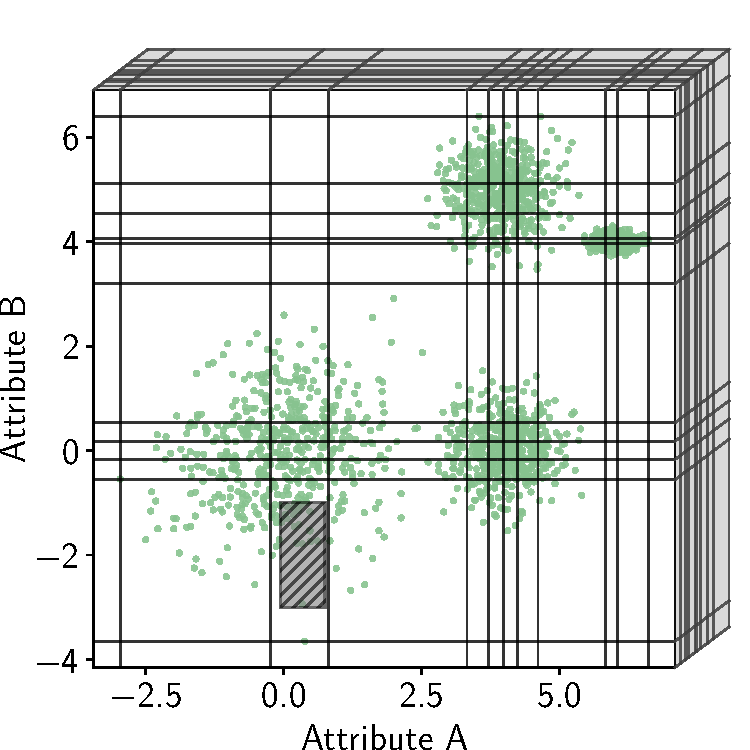
\includegraphics[width=\GridDataSpaceWidth]{../slides/figures/grid_index_3D}
                    };
                \node[anchor=north west, font=\GridPlanFigureFont\bfseries]
                    at (5,-5) {Team 5's data space:};

                % This is the same economical construction as the 3-D slide:
                % only exposed rims for the seven rear grids, two complete
                % foreground grids, and the final foreground grid split into
                % a 9 by 10 body plus a 1 by 10 row.
                \begin{scope}[shift={(84,-108)}, yshift=\GridCubeLift]
                    \def\gshift{1.4}
                    \def\goffset{5}
                    \def\goffsetY{14}
                    \def\cellsize{4.5}
                    \newcommand{\PosterLeafGrid}[5]{%
                        \pgfmathtruncatemacro{\PosterGridRows}{#2}%
                        \pgfmathtruncatemacro{\PosterGridColumns}{#3}%
                        \foreach \r in {1,...,#2}{%
                            \foreach \c in {1,...,#3}{%
                                \pgfmathsetmacro{\x}{(\c-1)*#4}
                                \pgfmathsetmacro{\y}{(\PosterGridRows-\r)*#5}
                                \node[gridcell, minimum width=#4mm, minimum height=#5mm,
                                    inner sep=0pt] at (\x,\y) {$\cdot$};%
                            }%
                        }%
                    }
                    \newcommand{\PosterLeafGridRim}[5]{%
                        \pgfmathtruncatemacro{\PosterGridRows}{#2}%
                        \pgfmathtruncatemacro{\PosterGridColumns}{#3}%
                        \foreach \c in {1,...,#3}{%
                            \pgfmathsetmacro{\x}{(\c-1)*#4}
                            \pgfmathsetmacro{\y}{(\PosterGridRows-1)*#5}
                            \node[gridcell, minimum width=#4mm, minimum height=#5mm,
                                inner sep=0pt] at (\x,\y) {$\cdot$};%
                        }%
                        \foreach \r in {2,...,\PosterGridRows}{%
                            \pgfmathsetmacro{\y}{(\PosterGridRows-\r)*#5}
                            \node[gridcell, minimum width=#4mm, minimum height=#5mm,
                                inner sep=0pt] at ({(\PosterGridColumns-1)*#4},\y) {$\cdot$};%
                        }%
                    }
                    \foreach \shift in {9,8,...,3} {
                        \begin{scope}[shift={({\goffset + \shift*\gshift},
                            {\goffsetY + \shift*\gshift})}]
                            \PosterLeafGridRim{grid}{10}{10}{\cellsize}{\cellsize}
                        \end{scope}
                    }
                    \foreach \shift in {2,1} {
                        \begin{scope}[shift={({\goffset + \shift*\gshift},
                            {\goffsetY + \shift*\gshift})}]
                            \PosterLeafGrid{grid}{10}{10}{\cellsize}{\cellsize}
                        \end{scope}
                    }
                    \begin{scope}[shift={(\goffset,{\goffsetY+\cellsize})}]
                        \PosterLeafGrid{grid}{9}{10}{\cellsize}{\cellsize}
                    \end{scope}
                    \begin{scope}[shift={(\goffset,\goffsetY)}]
                        \PosterLeafGrid{grid}{1}{10}{\cellsize}{\cellsize}
                    \end{scope}
                    \node[gridcell, fill=color5, minimum width=\cellsize mm,
                        minimum height=\cellsize mm, inner sep=0pt] (grid-reference-cell) at
                        ({\goffset+\cellsize},{\goffsetY}) {$\cdot$};
                    \node[font=\GridPlanFigureFont\bfseries]
                        at (-4,73) {Team 5's grid index:};
                    \node[overlay callout,fill=color5!60!white,anchor=pointer, inner sep=3pt,
                        draw=black!55, line width=0.7pt, 
                        callout relative pointer={(245:1.3cm)}, font=\DesignSpaceFigureTextFont]
                        at (grid-reference-cell.north)
                        {Relevant cell};
                    \node[overlay callout,fill=color2!70,anchor=pointer, inner sep=3pt,
                        draw=black,
                        callout relative pointer={(235:1.3cm)}, font=\DesignSpaceFigureTextFont]
                        at (55,70)
                        {$10^3$ cells};
                \end{scope}
                % Tune this source relative to the imported PDF's centre.
                \coordinate (grid-data-space-arrow-origin) at
                    ($(grid-data-space.center)+(\GridDataSpaceArrowXOffset,\GridDataSpaceArrowYOffset)$);
                \draw[halo arrow] (grid-data-space-arrow-origin) to[out=0,in=180]
                    (grid-reference-cell.west);

                \begin{scope}[shift={(88,-110)}]
                    \def\pagewidth{9}
                    \def\pageheight{15}
                    \def\pageheader{5}
                    \foreach \page in {0,...,6} {
                        \draw[draw=black!55, fill=white, line width=0.7pt]
                            ({\page*\pagewidth},0) rectangle ++(\pagewidth,\pageheight);
                        \fill[black!8] ({\page*\pagewidth},{\pageheight-\pageheader})
                            rectangle ++(\pagewidth,\pageheader);
                        \node[font=\scriptsize\bfseries] at
                            ({(\page+0.5)*\pagewidth},{\pageheight-0.5*\pageheader})
                            {\number\numexpr\page+1\relax};
                    }
                    \fill[\pagecolor] (0,1) rectangle ++(5.4,8);
                    \fill[color5] (\pagewidth,1) rectangle ++(7.2,8);
                    \coordinate (ssd-reference-segment) at (\pagewidth+3.6,6);
                    \fill[\pagecolor] (6*\pagewidth,1) rectangle ++(1.2,8);
                    \fill[\pagecolor] (4*\pagewidth,1) rectangle ++(12.8,8);
                    \fill[\pagecolor] (3*\pagewidth,1) rectangle ++(1.8,8);
                    \fill[\pagecolor] (2*\pagewidth,1) rectangle ++(0.9,8);
                    \node[font=\GridPlanFigureFont\bfseries, anchor=east] at (-5,8.5) {Storage Layout:};
                    \node[font=\GridPlanFigureFont\bfseries] at (7.2*\pagewidth,10) {$\ldots$};
                \end{scope}
                \draw[halo arrow] (grid-reference-cell.south) to[out=-90,in=90]
                    (ssd-reference-segment);
                \node[overlay callout,fill=color5!60!white,anchor=pointer, inner sep=3pt,
                        draw=black!55, line width=0.7pt, 
                        callout relative pointer={(215:3cm)}, font=\DesignSpaceFigureTextFont]
                        at (ssd-reference-segment.east)
                        {Compressed index ``leaf''};
            \end{tikzpicture}
        };
    \node[anchor=north west, inner sep=0pt] (complex-plan-figure)
        at ([xshift=\PlanXShift,yshift=-\GridFigureTopOffset]grid-plan-panel.north west) {
            \begin{tikzpicture}[remember picture, x=\PlanFigureUnit,y=\PlanFigureUnit]
                \tikzset{
                    complex plan flow/.style={->, >=Stealth, line width=0.9pt,
                        draw=black!80, line cap=round, shorten >=25pt},
                    complex plan leaf/.style={draw=black!55, fill=color4,
                        line width=0.65pt, rounded corners=1pt},
                    complex plan union/.style={draw=black!55, fill=color3,
                        line width=0.8pt, rounded corners=2pt, minimum width=1.0cm,
                        minimum height=0.65cm, font=\GridPlanFigureFont\bfseries},
                    complex plan intersect/.style={draw=color5, fill=color5!12,
                        line width=1pt, circle, minimum size=1.10cm, inner sep=0pt}
                }
                \pgfmathsetmacro{\complexbranchgap}{\ComplexPlanBranchGap/\PlanFigureUnit}
                \pgfmathsetmacro{\complexleafgap}{\ComplexPlanLeafGap/\PlanFigureUnit}
                \xdef\nextchildy{\ComplexPlanTopChildY}
                \xdef\allchildysum{0}
                \xdef\allchildcount{0}
                \foreach \branch/\childcount in {1/7,2/6,3/8,4/10,5/1} {
                    % The union is always centred at the arithmetic mean of
                    % its children's y coordinates, not at a fixed branch row.
                    \pgfmathsetmacro{\uniony}{\nextchildy-0.5*(\childcount-1)*\complexleafgap}
                    \ifnum\branch=5
                        \node[complex plan union, anchor=center, draw=black, fill=color5!30]
                            (complex-union-\branch) at (3.50,\uniony) {\ComplexPlanUnionSymbol};
                    \else
                        \node[complex plan union, anchor=center] (complex-union-\branch) at (3.50,\uniony) {\ComplexPlanUnionSymbol};
                    \fi
                    \foreach \leaf in {1,...,\childcount} {
                        \pgfmathsetmacro{\leafy}{\nextchildy-(\leaf-1)*\complexleafgap}
                        \draw[complex plan flow] (1.75,\leafy) -- (complex-union-\branch.center);
                        \ifnum\branch=5
                            \path[complex plan leaf, anchor=center, draw=black, fill=color5!30]
                                (0.95,\leafy-0.09) rectangle ++(0.32,0.18);
                            \coordinate (complex-relevant-leaf) at (1.11,\leafy);
                        \else
                            \path[complex plan leaf] (0.95,\leafy-0.09) rectangle ++(0.32,0.18);
                        \fi
                        \pgfmathparse{\allchildysum+\leafy}
                        \xdef\allchildysum{\pgfmathresult}
                        \pgfmathtruncatemacro{\updatedchildcount}{\allchildcount+1}
                        \xdef\allchildcount{\updatedchildcount}
                    }
                    \pgfmathparse{\nextchildy-(\childcount-1)*\complexleafgap-\complexbranchgap}
                    \xdef\nextchildy{\pgfmathresult}
                }
                \pgfmathsetmacro{\complexplanmeany}{\allchildysum/\allchildcount}
                \node[complex plan intersect] (complex-intersection) at (6.0,\complexplanmeany)
                    {$\displaystyle\bigcap$};
                \foreach \branch in {1,2,3,4,5} {
                    \draw[complex plan flow] (complex-union-\branch.east) -- (complex-intersection.center);
                }
                \node[draw=black!55, fill=color4, line width=0.8pt,
                    inner sep=4pt,
                    anchor=center,
                    rounded corners=1.5pt,
                    font=\GridPlanFigureFont\bfseries] (complex-candidates) at ($(complex-intersection.center)+(3.0,0)$) {Candidates};
                \draw[->, >=Stealth, line width=0.9pt,
                        draw=black!80, line cap=round, shorten >=4pt] (complex-intersection.east) -- (complex-candidates.west);
                % \node[font=\GridPlanFigureFont\bfseries, align=center, text=color5]
                %     at (1,9) {Many leaves in plan};
            \end{tikzpicture}
        };


    \node[draw=color3!70!black, rounded corners=4mm, line width=0.9pt,
        inner sep=\GridPlanGroupBoxPadding, fit=(complex-plan-figure)] (global-plan-box) {};
    \node[anchor=south east, fill=PanelFillColor, inner sep=2mm,
        font=\GridPlanFigureFont\bfseries]
        at ([xshift=-5mm,yshift=3mm]global-plan-box.south east) {Global execution plan};

    \node[anchor=north east, fill=color5!70!white, draw=black,
        line width=1pt, rounded corners=3mm, minimum width=\GridPlanNotesWidth,
        minimum height=\GridPlanNotesMinHeight, inner sep=5mm]
        at ([xshift=-\PanelPadding+0.8cm,
             yshift=-\GridPlanNotesTopOffset]grid-plan-panel.north east) {
            \begin{minipage}{\dimexpr\GridPlanNotesWidth+5mm\relax}
                \fontsize{14pt}{18pt}\selectfont
                \textbf{Challenge:}
                {\setlength{\leftmargini}{1.2em}
                \begin{itemize}
                    \item Need to account for per-leaf costs (''\textbf{overhead}'')!
                    \item Leaf count determines plan complexity
                    \item[$\mathbf{\Rightarrow}$] \textbf{Trade-off:} access volume vs. overhead
                \end{itemize}}
            \end{minipage}
        };

    %------- Row 3: Overhead vs. Volume + Runtime + Storage ------%
    \node[panel, minimum width=\ContentWidth, minimum height=\ContentRowHeight]
        (tradeoff-panel) at ([yshift=-\RowGap]selectivity-panel.south west) {};
    \node[panel heading] at ([xshift=\PanelPadding,yshift=-\PanelPadding]tradeoff-panel.north west) {
        \PanelHeading{Overhead vs. Volume / Runtime / Storage Consumption}
    };
    \node[anchor=north east, align=right, text=black!60]
        at ([xshift=-\DesignSpaceFootnoteRightInset,
             yshift=\DesignSpaceFootnoteTopInset]tradeoff-panel.south east) {
        \fontsize{20pt}{24pt}\selectfont
        \textsuperscript{*}\,\SI[mode=text]{153}{\giga\byte} LHCb data set / $\mathbf{16}$ attr. / $\mathbf{10^d}$ grids.
    };
    % Keep the figure nodes named: future explanatory callouts can anchor to
    % their edges without changing this three-column layout.
    \node[anchor=north west, inner sep=0pt] (volume-overhead-figure)
        at ([xshift=\PanelPadding,yshift=-\TradeoffFigureTopOffset]tradeoff-panel.north west) {
            \includegraphics[width=\TradeoffFigureWidth]{figures/generated/vol_vs_overhead_comparison}
        };
    \node[anchor=north west, inner sep=0pt] (runtime-figure)
        at ([xshift=\TradeoffFigureGap]volume-overhead-figure.north east) {
            \includegraphics[width=\TradeoffFigureWidth]{figures/generated/runtime_comparison}
        };
    \node[anchor=north west, inner sep=0pt] (storage-figure)
        at ([xshift=\TradeoffFigureGap]runtime-figure.north east) {
            \includegraphics[width=\TradeoffFigureWidth]{figures/generated/storage_comparison}
        };

    %% annotations:
    \node[overlay callout,fill=color5!70,anchor=pointer, inner sep=3pt,
        callout relative pointer={(235:1.3cm)}, font=\DesignSpaceFigureTextFont]
        at ([xshift=7cm,yshift=-2.75cm]runtime-figure.north) {Overhead costs\\are too high!};

    \node[overlay callout,fill=color5!70,anchor=pointer, inner sep=3pt,
        callout relative pointer={(315:1.5cm)}, font=\DesignSpaceFigureTextFont]
        at ([xshift=7cm,yshift=-5.75cm]storage-figure.north) {Grouping factor diminished\\$+$ compression deteriorated};
    %------- Row 4: Measured + Ideal Performance + Outlook ------%
    \node[panel, minimum width=\ContentWidth, minimum height=\ContentRowHeight]
        (performance-panel) at ([yshift=-\RowGap]tradeoff-panel.south west) {};
    \node[panel heading] at ([xshift=\PanelPadding,yshift=-\PanelPadding]performance-panel.north west) {
        \PanelHeading{Measured Performance vs. Ideal Performance (\& Outlook)}
    };
    \node[anchor=north east, align=right, text=black!60]
        at ([xshift=-\DesignSpaceFootnoteRightInset,
             yshift=-5mm]performance-panel.north east) {
        \fontsize{20pt}{24pt}\selectfont
        \textsuperscript{*}\,\SI[mode=text]{147}{\giga\byte} SDSS data set / $\mathbf{85}$ attr. / $\mathbf{8^5}$ grids \\%
        \fontsize{20pt}{24pt}\selectfont / Kioxia CM7-R 2TB (\SI[mode=text,per-mode=symbol]{14}{\giga\byte\per\second} sequ,%
        \SI[mode=text,per-mode=symbol]{8.2}{\giga\byte\per\second} rand).
    };
    \node[anchor=north west, inner sep=0pt] (scaling-comparison-figure)
        at ([xshift=\PanelPadding,yshift=-\PerformanceFigureTopOffset]performance-panel.north west) {
            \includegraphics[width=\PerformancePlotWidth]{figures/generated/dimensional_scaling_comparison}
        };
    \node[font=\SelectivityFigureFont\bfseries, text=black!65, align=center]
        at ([yshift=-0.0cm]scaling-comparison-figure.south) {measured performance};
                        
    \node[anchor=north east, inner sep=0pt] (bandwidth-figure)
        at ([xshift=-\PanelPadding,yshift=-\PerformanceFigureTopOffset]performance-panel.north east) {
            \includegraphics[width=\PerformancePlotWidth]{figures/generated/dimensional_scaling_io_bandwidth}
        };
    \node[font=\SelectivityFigureFont\bfseries, text=black!65, align=center]
        at ([yshift=-0.0cm]bandwidth-figure.south) {calculated performance};

    \draw[-{Stealth[round, length=42mm, width=80mm]}, line width=36mm,
        line cap=round, line join=round, draw=color3!80!white]
        ([xshift=16mm]scaling-comparison-figure.east)
        -- ([xshift=-8mm]bandwidth-figure.west);
    \node[anchor=center, inner sep=0pt] (performance-puzzle)
        at ($(scaling-comparison-figure.center)!0.5!(bandwidth-figure.center)$) {
            \resizebox{\PerformancePieWidth}{!}{%
                \begin{tikzpicture}
                    \useasboundingbox (-1.95,-1.75) rectangle (1.95,1.75);
                    \begin{scope}[xscale=1.2, yscale=0.85]
                        \begin{scope}[rotate=\PerformancePuzzleRotation]
                            \OutlookPuzzlePiece{PerformanceGeneralPieceColor}{135}{225}{-1}{1}{Operate\\at Scale}
                            \OutlookPuzzlePiece{PerformanceGeneralPieceColor}{225}{315}{-1}{1}{Execution\\Engine}
                            \OutlookPuzzlePiece{PerformanceDomainPieceColor}{-45}{45}{-1}{1}{Index\\Co-Design}
                            \OutlookPuzzlePiece{PerformanceDomainPieceColor}{45}{135}{-1}{1}{Team\\Composition}
                            \node[font=\PerformancePuzzleCenterFont\bfseries, text=black!65, align=center]
                                at (0,0.0) {Close\\the Gap};
                        \end{scope}
                        \path[postaction={decorate, decoration={text along path,
                            text align=center, text={|\PerformancePuzzleOuterLabelFont\bfseries\color{PerformanceGeneralLabelColor}|General}}}]
                            (160:1.8) arc[start angle=160, end angle=20, radius=1.8];
                        \path[postaction={decorate, decoration={text along path,
                            text align=center, text={|\PerformancePuzzleOuterLabelFont\bfseries\color{PerformanceDomainLabelColor}|Domain-specific}}}]
                            (200:1.92) arc[start angle=200, end angle=340, radius=1.92];
                        
                    \end{scope}
                \end{tikzpicture}%
            }
        };

    %------- Footer ------%
    \node[band, fill=FooterBandColor, minimum width=\paperwidth,
        minimum height=\FooterHeight, anchor=south west] (footer-band)
        at (current page.south west) {};
    \node[anchor=west] (bmftr-logo) at ([xshift=\PosterEdgeInset]footer-band.west) {
        
\includegraphics[height=\BmftrLogoHeight]{figures/generated/BMFTR_Logo}
    };
    \node[anchor=west] at ([xshift=8mm]bmftr-logo.east) {
        
\includegraphics[height=\LamarrLogoHeight]{figures/generated/lamarr}
    };
    \node[anchor=east] at ([xshift=-\PosterEdgeInset]footer-band.east) {
        \qrcode[height=\QrCodeHeight]{https://dbis.cs.tu-dortmund.de/publikationen/2025/index-intersection/}
    };
    

    \draw[-{Stealth[length=5mm,width=4mm]}, draw=black, line width=1.8pt,
    line cap=round, shorten >=2pt]
    ($(grid-index-figure.north west)+(\SsdReferenceLeafXOffset,\SsdReferenceLeafYOffset)$)
    to[out=0,in=180]
    ($(complex-plan-figure.north west)+(\ComplexPlanSingleLeafXOffset,\ComplexPlanSingleLeafYOffset)$);

\end{tikzpicture}

\end{document}